\documentclass{article}

\usepackage{pgfplots}
\usepackage{graphicx}
\usepackage[margin=0.75in, paperwidth=8.5in, paperheight=11in]{geometry}
\usepackage{setspace}
\usepackage{fancyvrb} % extended verbatim environments
\usepackage{framed}%To get shade behind text

\definecolor{shadecolor}{rgb}{0.9,0.9,0.9}%setting shade color


\begin{document}
\pagenumbering{gobble}

\doublespacing
\textbf{IB Computer Science }                        %%%(class number and section) 
 \hfill                             %%%(date of test)
$ {\bf Name:TaeyoungLee} \underline{\hspace{2.5in}}$(3 points)

\begin{centering}
\vspace{1cm}
\textbf{Exam 2}\\
\end{centering}
\vspace{1cm}
 

  
 $\bf{1)}$ Write the output of the following programs. (10 points each)
 
 \vspace{1cm}

  
 a.   \begin{verbatim}
 a=[0,1]
 for i in range(1,5):
       a=a+[a[i]+a[i-1]]
 print a
 \end{verbatim}
 \vspace{1cm}
 \begin{verbatim}
 [0,1,1,2,3,5]
 \end{verbatim}
 b.  \begin{verbatim}
 a=[]
 for i in range(4):
     b=[]
     for x in range(3):
         b=b+[i+2*x]
     a=a+[b]
 print a
 \end{verbatim}
 \vspace{1cm}
 
 \begin{verbatim}
 [[0,2,4],[1,3,5],[2,4,6],[3,5,7]]
 \end{verbatim}

 c.  \begin{verbatim}
 a=[1,3,4,2,8]
 b=[]
 for i in range(len(a)-1):
     b=b+[a[i+1]-a[i]]
 print b
 \end{verbatim}
 \begin{verbatim}
 [2,1,­‐2,6]
 \end{verbatim}
  \newpage
  
  $\bf{2)}$ Write the output of the following programs. (10 points each)
  
  a.  Write a program that prints the sum of 100 random number between 0 and 1. 
  \begin{verbatim}
  Import random
  S=0
  For i in range(100):
	  S=s+random.uniform(0,1)
  Print s
  \end{verbatim}
  b.  Write a program that prints the average value of an array "a". 
  \begin{verbatim}
a=[n,n+1,n+2,n+3,n+4,n+5……]
print sum(a)/len(a)
  \end{verbatim}
  c.  Write a program that builds a 10 by 10 checkerboard array of ones and zeros.
	\begin{verbatim}
	Import random
	xx=[]
	for i in range(10):
	r=xx+[range(10)]
	b=range(10)
	t=3.0
	for j in range(10):
	for i in range(10):
		if random.uniform(0,10)<t:
			r[i][j]=1
		else:
			r[i][j]=0
	print r
	\end{verbatim}
  
  
  
    \newpage
  
  $\bf{3)}$  Draw the output of the following program. (20 points)
  \begin{verbatim}
from graphics import *

win=GraphWin()
win.setCoords(-10,-10,10,10)

for i in range(1,6):
    circ=Circle(Point(i,i),(2**0.5) * i)
    rec=Rectangle(Point(-i,-i),Point(0,0))
    t = Text(Point(-5,9-i), "yo")
    circ.draw(win)
    rec.draw(win)
    t.draw(win)
    \end{verbatim}
    \begin{figure}
    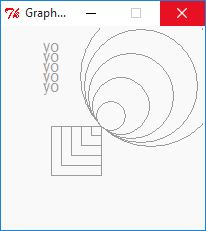
\includegraphics[width=40mm]{midterm_makeup.jpg}
    \end{figure}
   
  \newpage
  
  $\bf{4)}$ Perform the following conversions. (10 points each)
  \vspace{0.5cm}
  
   a. Convert the Base5 number 432 to Base10. 
   \begin{verbatim}
   97
   \end{verbatim}
  
  b. Convert the binary number 1010001 to Base10. 
  \begin{verbatim}
  81
  \end{verbatim}
  c. Convert the Base10 number 532 to Base5.
  \begin{verbatim}
  4112
  \end{verbatim}
  

 
\end{document}